\documentclass[12pt]{article}

\title{\vspace{-3em}PHYS 161a HW 1}
\author{Michael Cardiff}
\date{\today}

%% science symbols 
\usepackage{amsmath}
\usepackage{amssymb}
\usepackage{physics}
\usepackage{slashed}

%% general pretty stuff
\usepackage{bm}
\usepackage{enumitem}
\usepackage{float}
\usepackage{graphicx}
\usepackage[margin=1in]{geometry}
\usepackage[labelfont=bf]{caption}
\usepackage{tikz}


% figures
\graphicspath{ {./figs/} }

\newcommand{\fig}[3]
{
  \begin{figure}[H]
    \centering
    \includegraphics[width=#1cm]{#2}
    \caption{#3}
  \end{figure}
}

\newcommand{\figref}[4]
{
  \begin{figure}[H]
    \centering
    \includegraphics[width=#1cm]{#2}
    \caption{#3}
    \label{#4}
  \end{figure}
}

\newcommand*\circled[1]{\tikz[baseline=(char.base)]{
            \node[shape=circle,draw,inner sep=2pt] (char) {#1};}}
\renewcommand{\L}{\mathcal{L}}
\renewcommand{\vb}[1]{\bm{#1}}
\newcommand{\D}{\partial}
\newcommand{\munu}{{\mu\nu}}
\newcommand{\sla}[1]{\slashed{#1}}
\newcommand{\infint}{\int_{-\infty}^\infty}
\newcommand{\veps}{\varepsilon}

\begin{document}
\maketitle

\section*{Problem 1}
The full integral expands to:
\begin{align*}
  \int_{-\infty}^{\infty}\frac{\phi(x)}{x+i\epsilon}\dd{x}
  &=\infint\frac{\phi(x)-\phi(0)+\phi(0)}{x+i\epsilon}\dd{x}\\
  &=\infint\frac{\phi(x)-\phi(0)}{x+i\epsilon}\dd{x}+
  \infint\frac{\phi(0)}{x+i\epsilon}\dd{x}\\
  &=\circled{1}+\circled{2}
\end{align*}
The integral \circled{1}, when we take the limit as $\epsilon\to0$ is the action of the principal value integral of $\frac1x$:
\begin{align*}
  \lim_{\epsilon\to0}\circled{1}&=\infint\frac{\phi(x)-\phi(0)}{x}\dd{x}\\
  &=\ip{\mathrm{pv}\qty(\frac1x)}{\phi}
\end{align*}
The integral \circled{2}:
\begin{align*}
  \circled{2}&=\infint\frac{\phi(0)}{x+i\epsilon}\dd{x}\\
  &=\infint\frac{\phi(0)(x-i\varepsilon)}{x^2+\epsilon^2}\dd{x}\\
  &=\phi(0)\infint\frac{x}{x^2+\epsilon^2}\dd{x}
  -i\epsilon\phi(0)\infint\frac{1}{x^2+\epsilon^2}\dd{x}
\end{align*}
The first integral has the form of $\frac{\dd{f}}{f}$, which is a natural log, which would evaluate to $0$. The second integral is a standard one whose result is inverse tangent, however it is ill defined at $\pm\infty$:
\begin{align*}
  \circled{2}&=-i\epsilon\phi(0)\lim_{q\to\infty}
  \int_{-q}^q\frac{\dd{x}}{x^2+\epsilon^2}
  =-i\epsilon\phi(0)\eval{\frac{1}{\epsilon}\arctan\frac{x}{\epsilon}}_{-q}^q\\
  &=2i\phi(0)\frac{\pi}{2}=\pi i\phi(0)
\end{align*}
Taking the limit as $\epsilon\to0$ yields a multiplier of the $\phi(0)$:
\begin{align*}
  \circled{2}&=\pi i\ip{\delta}{\phi}
\end{align*}
Thus the action of $\delta^+$ is:
\begin{align*}
  \ip{\delta^+}{\phi}=\frac12\ip{\delta}{\phi}
  -\frac{1}{2\pi i}\ip{\mathrm{pv}\qty(\frac1x)}{\phi}
\end{align*}
Therefore:
\begin{align}
  \boxed{
    \delta^+(x)=\frac12\delta(x)-\frac1{2\pi i}\mathrm{pv}\qty(\frac1x)
  }
\end{align}
\section*{Problem 2}
Define this commutator-like operation on a distribution:
\begin{align*}
  \ip{\comm{x}{\dv{x}}T}{\phi}&=\ip{x\dv{T}{x}}{\phi}-\ip{\dv{x}(xT)}{\phi}\\
  &=\circled{1}-\circled{2}
\end{align*}
The first one:
\begin{align*}
  \circled{1}&=\int\qty(x\dv{f}{x})\phi(x)\dd{x}\\
  &=\int\dv{f}{x}\qty(x\phi(x))\dd{x}\\
  &=\ip{T'}{x\phi(x)}\\
  &=-\ip{T}{\{x\phi(x)\}'}
\end{align*}
Where the $\{\}$ denotes the classical derivative:
\begin{align*}
  \circled{1}&=-\ip{T}{\{x\phi(x)\}'}\\
  &=-\ip{T}{x\phi'(x)+\phi(x)}
\end{align*}
The second integral:
\begin{align*}
  \circled{2}&=\ip{\dv{(xT)}{x}}{\phi}=-\ip{xT}{\phi'(x)}\\
  &=-\ip{T}{x\phi'(x)}
\end{align*}
Then combining with $\circled{1}$:
\begin{align*}
  \circled{1}-\circled{2}&=-\ip{T}{x\phi'(x)+\phi(x)}+\ip{T}{x\phi'(x)}\\
  &=\ip{T}{-x\phi'(x)-\phi(x)+x\phi'(x)}\\
  &=\ip{T}{-\phi(x)}
\end{align*}
Hence we can use linearity of the first derivative again:
\begin{align*}
  \ip{\comm{x}{\dv{x}}T}{\phi}=-\ip{T}{\phi}
\end{align*}
Hence we can conclude:
\begin{align}
  \boxed{\comm{x}{\dv{x}}T=-T}
\end{align}
\section*{Problem 3}
The function $f(x)=\log\abs{x}$ is locally integrable, so we can define it as a distribution, such that its distributional derivative is:
\begin{align*}
  \ip{T_f'}{\phi}=-\ip{T_f}{\phi'}
\end{align*}
Hence we need to calculate:
\begin{align*}
  -\ip{\log\abs{x}}{\phi'}
\end{align*}
Which we can find is:
\begin{align*}
  \ip{\qty[\log\abs{x}]'}{\phi}&=-\lim_{\epsilon\to0}
  \qty(\int_{-\infty}^{-\epsilon}\log\abs{x}\phi'(x)\dd{x}
  +\int_\epsilon^\infty\log\abs{x}\phi'(x)\dd{x})
\end{align*}
Since none of these integrals will be evaluated at $0$, the classical derivative of $\log\abs{x}$ is valid, so it makes sense to do integration by parts in each of the separate integrals
\begin{align*}
  \ip{\qty[\log\abs{x}]'}{\phi}&=-\lim_{\epsilon\to0}
  \qty(
  \eval{\log\abs{x}\phi(x)}_{-\infty}^{-\epsilon}
  -\int_{\infty}^{-\epsilon}\frac{\phi(x)}{x}\dd{x}
  +\eval{\log\abs{x}\phi(x)}_\epsilon^\infty
  -\int_\epsilon^\infty\frac{\phi(x)}{x}\dd{x})
\end{align*}
The two functions which must be evaluated:
\begin{align*}
  \eval{\log\abs{x}\phi(x)}_{-\infty}^{-\epsilon}+
  \eval{\log\abs{x}\phi(x)}_\epsilon^\infty=
  \log\epsilon\qty(\phi(-\epsilon)+\phi(\epsilon))
\end{align*}
Expanding $\phi$ in terms of $\epsilon$ yields canceling linear terms, so the limit as $\epsilon$ is small means we can keep linear terms, so these terms are $0$. The remainder is simply the definition of the principle value integral:
\begin{align*}
  \ip{\qty[\log\abs{x}]'}{\phi}&=-\lim_{\epsilon\to0}
  \qty(\int_{-\infty}^{-\epsilon}\frac{\phi(x)}{x}\dd{x}+
  \int_{\epsilon}^{\infty}\frac{\phi(x)}{x}\dd{x})
  \equiv\ip{\mathrm{pv}\qty(\frac1x)}{\phi}
\end{align*}
Therefore we can conclude:
\begin{align}
  \boxed{
    \qty[\log\abs{x}]'=\mathrm{pv}\qty(\frac1x)
  }
\end{align}
\section*{Problem 4}
\subsection*{Part 1}
We start with the following notions of the dot product and cross product in terms of indices:
\begin{gather*}
  \vb{a}\vdot\vb{b}\equiv a_ib_i=\delta_{ij}a_ib_j\\
  (\vb{a}\times\vb{b})_i\equiv\varepsilon_{ijk}a_jb_k
\end{gather*}
Note that Einstein convention is used, repeated indices are summed over.

I would like to go from the right hand side to the left, we can get that:
\begin{align*}
  \vb{a}\vdot\vb{b}&=a_ib_i\\
  \vb{\sigma}\vdot(\vb{a}\times\vb{b})&=\sigma_i\qty(\vb{a}\times\vb{b})_i\\
  &=\sigma_i\varepsilon_{ijk}a_jb_k
\end{align*}
In the identity, we have the second quantity times $i$:
\begin{align*}
  i\varepsilon_{ijk}\sigma_ia_jb_k
\end{align*}
Note $\varepsilon$ is the totally antisymmetric tensor, so cyclic permutations of its indices are permitted without changing value, in this case we can swap $i$ to the end to find:
\begin{align*}
  i\varepsilon_{ijk}\sigma_ia_jb_k=(i\varepsilon_{jki}\sigma_i)a_jb_k
\end{align*}
The provided identity gives:
\begin{align*}
  i\varepsilon_{jki}\sigma_i=\sigma_j\sigma_k-\delta_{jk}
\end{align*}
Hence:
\begin{align*}
  i\varepsilon_{jki}\sigma_ia_jb_k&=(\sigma_j\sigma_k-\delta_{jk})a_jb_k\\
  &=(\sigma_ja_j)(\sigma_kb_k)-\delta_{jk}a_jb_k\\
  &=(\sigma_ja_j)(\sigma_kb_k)-a_kb_k
\end{align*}
Combining with the first dot product to get the identity:
\begin{align*}
  (\sigma_ja_j)(\sigma_kb_k)-a_kb_k=
  (\vb{\sigma}\vdot\vb{a})(\vb{\sigma}\vdot\vb{b})
  +\vb{a}\vdot\vb{b}-\vb{a}\vdot\vb{b}
\end{align*}
Giving our identity:
\begin{align}
  \boxed{
    (\vb{\sigma}\vdot\vb{a})(\vb{\sigma}\vdot\vb{b})=
    \vb{a}\vdot\vb{b}+i\vb{\sigma}\vdot(\vb{a}\times\vb{b})
  }
\end{align}
\subsection*{Part 2}
\subsubsection*{Part a}
The original argument to the integral is:
\begin{align*}
  \vb{F}\vdot\vb{G}=\grad{\phi}\vdot\vb{G}
\end{align*}
However since $\div{\vb{G}}=0$, we can add a scalar multiple of it to get the same result:
\begin{align*}
  \grad{\phi}\vdot\vb{G}+\phi\div{\vb{G}}=\div{(\phi\vb{G})}
\end{align*}
Which is the divergence scalar multiplication product rule. Then under the integral we can use one of the vector calculus integral theorems:
\begin{align*}
  \int\div{(\phi\vb{G})}\dd[3]{r}=\oint_S\phi\vb{G}\vdot\dd{\vb{S}}
\end{align*}
This should go to $0$, as $\phi\abs{\vb{G}}$ goes to $0$ faster than $r^{-2}$, which already goes to $0$:
\begin{align}
  \boxed{\int\dd[3]{r}\vb{F}\vdot\vb{G}=0}
\end{align}
\subsubsection*{Part b}
Using $\vb{F}$ as a gradient again we can use the cross product product rule to get:
\begin{align*}
  \curl{(\phi\vb{G})}=(\grad{\phi})\times\vb{G}+\phi(\curl{\vb{G}})
\end{align*}
The second term goes to $0$, meaning the integral is:
\begin{align*}
  \int(\grad{\phi})\times\vb{G}\dd[3]{r}=\int\curl{(\phi\vb{G})}\dd[3]{r}
\end{align*}
Using a similar vector calculus integral identity we can get:
\begin{align*}
  \int\curl{(\phi\vb{G})}\dd[3]{r}=\oint_S(\phi\vb{G})\times\dd{\vb{S}}
\end{align*}
For the same reasons as part a, this should go to $0$:
\begin{align}
  \boxed{\int\dd[3]{r}\vb{F}\times\vb{G}=0}
\end{align}
\subsubsection*{Part c}
I believe the intention is to show that you can decompose an integral into its normal and tangent components, however this is in an integral, so it is a bit different. We should take $\vb{G}=\vb{r}$. The index composition of the divergence gives:
\begin{align*}
  \D_j(P_j\vb{r})=(\div{\vb{P}})\vb{r}+(P_j\D_j)\vb{r}
\end{align*}
By the product rule. The derivative of the $\vb{r}$ vector is one of the cartesian coordinates, so this just a reconstruction of the original vector $\vb{P}$:
\begin{align*}
  \D_j(P_j\vb{r})=(\div{\vb{P}})\vb{r}+\vb{P}
\end{align*}
Integrating both sides over a volume $V$
\begin{align*}
  \int_V\D_j(P_j\vb{r})\dd[3]{r}=\int_V(\div{\vb{P}})\vb{r}\dd[3]{r}
  +\int_V\vb{P}\dd[3]{r}
\end{align*}
The left hand side is a divergence, and we can use one of those handy vector calculus integral identities to turn it into an integral over a surface:
\begin{align*}
  \int_V\D_j(P_j\vb{r})\dd[3]{r}&=\int_V(\div{\vb{P}})\vb{r}\dd[3]{r}\\
  &=\int_S\vb{r}\qty(\vu{n}\vdot\vb{P})\dd{S}
\end{align*}
Hence some algebra gives the desired result:
\begin{align}
  \boxed{
    \int_V\vb{P}\dd[3]{r}=-\int_V\vb{r}\qty(\div{\vb{P}})\dd[3]{r}
    +\int_S(\vu{n}\vdot\vb{P})\vb{r}\dd{S}
  }
\end{align}
\section*{Problem 5}
We want to consider a point $P$ a normal distance $d=0.5$ away from a plane of charge. In order to calculate the field due to the charges within an inch, we need to draw a triangle:
\begin{figure}[H]
  \centering
  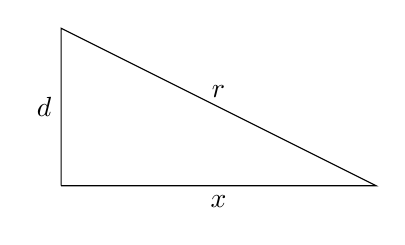
\begin{tikzpicture}
    \draw (0,0) -- (0,2) node[midway,left] {$d$}
    -- (4,0) node[midway,above] {$r$}
    -- (0,0) node[midway,below] {$x$};
\end{tikzpicture}
  \caption{Toy Model}
\end{figure}
In the figure, the distance $x$ is to be integrated through, and $d=0.5$. We must calculate the $\vb{r}-\vb{r}'$ in order to integrate Coulomb's law properly:
\begin{align*}
  \vb{r}&=d\vu{y}\\
  \vb{r}'&=x\vu{x}\\
  \vb{r}-\vb{r}'&=-x\vu{x}+d\vu{x}\\
  \qty(\vb{r}-\vb{r}')^2&=x^2+d^2
\end{align*}
Note that an integral over the space we want is:
\begin{align*}
  \int_{1-in}=\int_0^1\int_0^{2\pi}\dd{\phi}\dd{x}
\end{align*}
Which is some odd version of cylindrical coordinates.

Coulomb's law tells us:
\begin{align*}
  \dd{E}=\frac1{4\pi\varepsilon_0}\frac{\dd{q}}{\qty(\vb{r}-\vb{r}')^2}
\end{align*}
In this case $\dd{q}=\sigma\dd{x}\dd{\phi}$, integrating:
\begin{align*}
  E=\frac{\sigma}{4\pi\varepsilon_0}\int_0^1\int_0^{2\pi}
  \frac{1}{x^2+d^2}\dd{\phi}\dd{x}
\end{align*}
This is a fairly elementary integral:
\begin{align*}
  E&=\frac{\sigma}{4\pi\veps_0}2\pi\eval{\frac{\arctan\frac{x}{d}}{d}}_0^1\\
  &=\frac{\sigma}{2\veps_0d}\arctan\frac1d
\end{align*}
At small $d$ the arctan term combined with the $1/d$ goes to a $1$\footnote{This was due to a mathematica series expansion}
This all cancels out to:
\begin{align}
  \boxed{E_{1-in}=\frac{\sigma}{4\veps_0}}
\end{align}
Which is one half of the total value!
\end{document}